\chapter{Experimental evaluation} \label{experiments}
Three case studies: a pilot study, a classroom case study, and a public data case study will be conducted in order to empirically evaluate capabilities and performance of the Hackystat Trajectory framework. A pilot study is ongoing along with development of the framework and some of the results discussed in this chapter.

The primary goal of these studies is to assess the ability of the framework to reproduce well known recurrent behavioral patterns (for example TDD), as well as the ability to discover novel ones. As the secondary goal, I see the classification and extension of the current Hackystat sensors family in order to improve the system performance. It is quite possible that some of the currently collected sensor data will be excluded from the Trajectory Analysis datasets, while some new ones will be designed and developed in order to capture important features from software process. 

\section{Pilot study}\label{pilot.evaluation}
In order to demonstrate the ability of the current framework implementation to perform telemetry indexing and temporal recurrent patterns extraction, I have conducted two pilot experiments discussed next. 

\begin{figure}[tbp]
   \centering
   \includegraphics[height=185mm]{cluster_streams.eps}
   \caption{Clustering of telemetry streams for classroom pilot dataset using symbolic approximation and vectors of motif frequencies. While it seems to be meaningful to find correlation between \textit{UnitTest\_Failure} and \textit{CodeIssue} streams unit test, this grouping happened due to the similarity of behavior pattern - short, hight in amplitude bursts; but note, there is no correlation in time.}
   \label{fig:cluster_streams}
\end{figure}

\subsection{Clustering of the Hackystat Telemetry streams}
The main purpose of the first pilot study was to evaluate the ability of PAA and SAX approximations to capture recurrent temporal patterns in telemetry streams. Knowing about usually misleading results of time-series clustering \cite{citeulike:227029}, I did not expect to capture much interesting facts, nevertheless the results were encouraging.

For pilot study I used real data collected during the Spring'09 software engineering class. This dataset represents Hackystat metrics collected during sixty days of a classroom project development conducted by eight students. The following clustering experiments were conducted using the distance between vectors of motif frequencies:
\begin{itemize}
	\item Clustering of software process related telemetry streams collected from individual developers. I was able to group developers with the similar behavioral patterns within clusters, which indicates the correctness of the classification approach.
	\item Clustering of software product-related telemetry streams by using shared motif frequencies. As a result of this experiment, I was able to group telemetry streams, but while stream groups look intuitively meaningful, close examination of the streams indicates that this grouping happened just because of the method applied. The results indicate that instead of using just motif frequencies, some temporal ordering should be taken into account.
\end{itemize}

\subsection{Sequential patterns search}
The second pilot study, aiming at discovery of sequential patterns, was also conducted using real data from my own concurrent development of two software projects. While working on the Hackystat Trajectory framework, I made decision to split the code into two parts: an algorithm implementation library that I named JMotif, and the user-interface part called TrajectoryBrowser. While this decision simplified development, it introduced a heavy dependency of TrajectoryBrowser on the JMotif API, which provides variations of DTW, PAA and SAX algorithms along with defining data structures for indexing and clustering. As a result of iterative and incremental pattern in my development, I changed the JMotif public API three times, which consequently involved extensive refactoring in the ProjectBrowser code. This dependency can be clearly seen from observing DevTime streams at Figure \ref{fig:sequential_growth} panel $a$. 

\begin{figure}[tbp]
   \centering
   \includegraphics[height=80mm]{sequential_growth.eps}
   \caption{The illustration of finding of sequential $growth \; pattern$ in two DevTime telemetry streams. Panel $a$: The Hackystat ProjectBrowser showing telemetry streams. Panel $b$: the TrajectoryBrowser showing same telemetry streams along with identified pattern. Panel $c$: the symbolic representation of streams with highlighted pattern.}
   \label{fig:sequential_growth}
\end{figure}

In order to capture this dependency pattern in two Telemetry streams, representing daily amount of development time spent on the TrajectoryBrowser and JMotif projects, I defined a synthetic \textit{growth pattern} as the large positive delta value between previous and current day effort. By transforming Telemetry streams with this simple rule in the symbolic form, I obtained a two dimensional symbolic time series, where letter $G$ represents a growth pattern, see Figure \ref{fig:sequential_growth} panel $c$. I have defined a formal rule for \textit{sequential growth} pattern as the pattern like $G_{JMotif}\; \rightarrow \; G_{TrajectoryBrowser}$ where distance between these $G$s is less than three days. By application of this rule I identified a pattern which exactly corresponds to my experience.
